\chapter{Training data of CFD results to train surrogate model}
In our case, 80 DOEs are generated and steady state 3D CFD analysis has been performed for these 80 shapes. The solver parameters used are as follows:
\begin{table}[H]
	\caption{Flow conditions and solver parametres for all DOE shapes}
	\label{Flow conditions and solver parametres for all DOE shapes}
	\centering
	\begin{tabular}{ll}
		\hline \hline
		Parameters & Value \\ 
		\hline \hline
		Reynolds number based on volume Re & $ 3.01 \ast 10^6 $ \\
		Pressure, N/m2 & 87500 \\
		Density, Kg/m3 & 1.057 \\
		Speed, m/s & 51 \\
		Mesh & Hexahedral mesh using blockMesh and snappyHexMesh \\
		Solver & SimpleFOAM (Incompressible steady state solver) \\
		Turbulent..? & Yes \\
		Turbulence model & K-Omega SST \\
		\hline \hline
	\end{tabular}
\end{table}
\section{Grid Convergence study}

Effect of grid size on the overall results by  changing the number of cells in self similar mesh has been carried out. Below is the plot of variation of pressure and viscous drag with number of cells for a simulation. As mentioned by \cite{Suman2011} , when the percentage change in the values is less than 5 \%, then the solution is reported to have grid convergence.

\begin{table}[H]
	\caption{Grid convergence study}
	\label{Grid convergence table}
	\centering
	\begin{tabular}{ccc}
		\hline \hline
		Cells & Pressure Drag (N) & Viscous Drag (N) \\
		\hline \hline
		376380 & 1.1  & 11.02 \\
		604375  & 2.2  & 11.68 \\
		840565  & 2.02  & 12.1 \\
		994864  & 2.09  & 12.24 \\
		1563471  & 2.12 & 12.5 \\
		\hline \hline
	\end{tabular}
\end{table}

\begin{figure}[H]
	\centering
	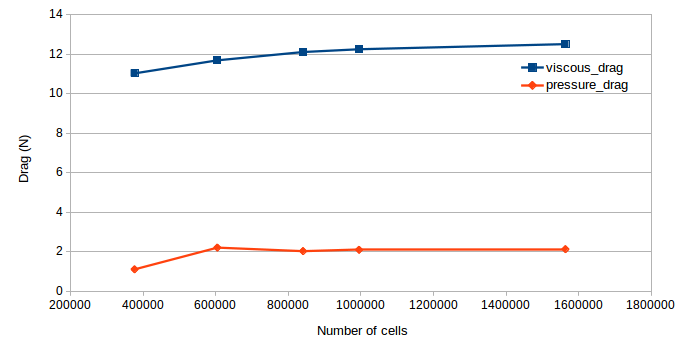
\includegraphics[width=300 pt]{surrogate_model_CFD_results/Grid_convergence.png}
	\caption{Variation of pressure and viscous drag with number of cells}
	\label{Grid convergence plot} %      only if needed
\end{figure}


